%%%%%%%%%%%%%%%%%%%%%%%%%%%%%%%%%
%
%       EXERCÍCIO
%
%%%%%%%%%%%%%%%%%%%%%%%%%%%%%%%%%

\ifdefstring{\atividade}{prova}{%
    \ifdefstring{\modo}{objetivo}{%
        \renewcommand{\valorquestao}{\ValorQObj\ ponto}
    }{%
        \renewcommand{\valorquestao}{\ValorQDisc\ pontos}
    }%
}%

\begin{exercicioBanco}[\valorquestao]
Os gráficos abaixo representam as funções receita mensal \(R(x)\) e custo mensal \(C(x)\) de um produto fabricado por uma empresa, em que \(x\) é a quantidade produzida e vendida. Responda qual é o lucro obtido ao se produzir
e vender \(1350\) unidades por mês.

\begin{center}
    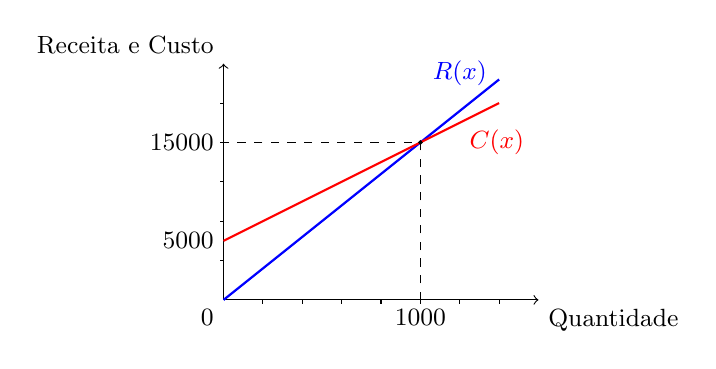
\begin{tikzpicture}[scale=0.5]

        % Eixos
        \draw[->] (0,0) -- (8,0) node[below right] {\small Quantidade};
        \draw[->] (0,0) -- (0,6) node[above left] {\small Receita e Custo};

        % R(x) = 15x (normalizado para caber melhor)
        \draw[domain=0:7, smooth, variable=\x, blue, thick] 
            plot ({\x}, {0.8*\x});
        \node[blue, above] at (6,5.2) {\small \(R(x)\)};

        % C(x) = 10x + 5000 (também reescalado)
        \draw[domain=0:7, smooth, variable=\x, red, thick] 
            plot ({\x}, {0.5*\x + 1.5});
        \node[red, right] at (6,4) {\small \(C(x)\)};

        % Ponto de interseção (aproximado)
        \filldraw (5,4) circle (1.2pt);
        
        \draw[dashed] (5,0) -- (5,4) -- (0,4);
        \node[below] at (5,0) {\small \(1000\)};
        \node[left] at (0,4) {\small \(15000\)};
        \node[below left] at (0,0) {\small \(0\)};
        \node[left] at (0,1.5) {\small \(5000\)};

        % Marcas nos eixos (opcional)
        \foreach \x in {1,2,3,4,5,6,7}
            \draw (\x,0) -- (\x,-0.1);

        \foreach \y in {1,2,3,4,5}
            \draw (0,\y) -- (-0.1,\y);

    \end{tikzpicture}
\end{center}

% Define as alternativas
\newcommand{\alternativas}{%
    \begin{center}
        \begin{tabularx}{\textwidth}{XXXXX}
            (a) R\$ \(6750{,}00\). &
            (b) R\$ \(2500{,}00\). &
            (c) R\$ \(2000{,}00\). &
            (d) R\$ \(1750{,}00\). &
            (e) R\$ \(1500{,}00\).
        \end{tabularx}
    \end{center}
}

% Resposta correta
\newcommand{\resposta}{D}

% Lógica condicional para exibição
\ifdefstring{\atividade}{lista}{%
    \alternativas
    \vspace{0.5em}
    
    \noindent\textbf{Resposta:} letra \textbf{\resposta}.
}{%
    \ifdefstring{\modo}{objetivo}{%
        \alternativas
    }{%
        % modo = discursiva → não mostra alternativas
    }
}
\end{exercicioBanco}

